\documentclass[11pt]{article}
\usepackage[utf8]{inputenc}
\usepackage[T1]{fontenc}
% Unicode symbols of the Lean source, so that it can be quoted verbatim
\DeclareUnicodeCharacter{2286}{\ensuremath{\subseteq}}
\DeclareUnicodeCharacter{2192}{\ensuremath{\to}}
\DeclareUnicodeCharacter{211D}{\ensuremath{\mathbb{R}}}
\DeclareUnicodeCharacter{2200}{\ensuremath{\forall}}
\DeclareUnicodeCharacter{2203}{\ensuremath{\exists}}
\DeclareUnicodeCharacter{2264}{\ensuremath{\le}}
\DeclareUnicodeCharacter{2227}{\ensuremath{\wedge}}
\DeclareUnicodeCharacter{2243}{\ensuremath{\simeq}}
\DeclareUnicodeCharacter{1D62}{\ensuremath{_i}}
\DeclareUnicodeCharacter{2194}{\ensuremath{\leftrightarrow}}
\usepackage{amsmath,amssymb,amsthm,mathtools}
\usepackage{tikz}
\usepackage[margin=1in]{geometry}
\setlength{\emergencystretch}{3em}
\usepackage[colorlinks=true,linkcolor=blue,citecolor=blue,urlcolor=blue]{hyperref}

\newtheorem{theorem}{Theorem}[section]
\newtheorem{lemma}[theorem]{Lemma}
\newtheorem{proposition}[theorem]{Proposition}
\newtheorem{corollary}[theorem]{Corollary}
\theoremstyle{definition}
\newtheorem{definition}[theorem]{Definition}
\theoremstyle{remark}
\newtheorem{remark}[theorem]{Remark}
\newtheorem{example}[theorem]{Example}

\newcommand{\R}{\mathbb{R}}
\newcommand{\Ort}{\mathrm{O}(3)}
\newcommand{\Fit}{\operatorname{Fit}}
\newcommand{\NC}{\operatorname{NC}}
\newcommand{\sgn}{\operatorname{sgn}}
\DeclarePairedDelimiter{\abs}{\lvert}{\rvert}
\DeclarePairedDelimiter{\norm}{\lVert}{\rVert}

\title{When does a box fit into a box?\\ An explicit criterion with a formal proof}
\author{Mikhail Levit}
\date{September 27, 2026}

\begin{document}


\maketitle

\begin{abstract}
We give a necessary and sufficient condition, in closed form, for a rectangular box with edges
$q_1,q_2,q_3\ge 0$ to fit, after an arbitrary rigid motion, into a rectangular box with edges
$p_1,p_2,p_3>0$. The condition is a disjunction of nine explicit checks, each consisting of two
planar tests expressed by a formula with a single square root. The key geometric fact is that if a
box fits at all, it fits in a position where one of its edges is perpendicular to one of the axes of
the container; we prove this by showing that at any other position all three widths of the box can be
decreased simultaneously. The problem was posed by Garnett in 1923 and was described by Jerrard and
Wetzel in 2004 as an instance of a general unsolved fitting problem for boxes in
higher dimensions. The main theorem has been verified in the Lean~4 proof assistant with the Mathlib
library, together with the analogous criterion for strict fitting (without touching the container),
which is not obtained by merely making the inequalities strict. The criterion is constructive: when
the box fits, it yields an explicit rotation. An implementation decides fitting and produces a
placement in about $20$ microseconds, three to four orders of magnitude faster than a multi-start
local numerical search over rotations, and without its false negative answers near the boundary.
\end{abstract}

\section{Introduction}

Let $P=[0,p_1]\times[0,p_2]\times[0,p_3]$ with $p_i>0$ and $Q=[0,q_1]\times[0,q_2]\times[0,q_3]$ with
$q_j\ge 0$. We say that $Q$ \emph{fits into} $P$ if $f(Q)\subseteq P$ for some isometry $f$ of $\R^3$.
The question of when this happens was posed by F.~M.~Garnett in 1923
\cite{Garnett1923}; W.~B.~Carver \cite{Carver1925} gave a partial answer, assuming without proof that
in an optimal position all vertices of $Q$ lie on faces of $P$. The planar analogue, a rectangle in a
rectangle, was settled by Carver in 1957 \cite{Carver1957} (see also Wetzel \cite{Wetzel2000}).
Jerrard and Wetzel \cite[p.~22]{JerrardWetzel2004} describe the three-dimensional question as an
instance of a ``general unsolved fitting problem for boxes in higher dimensions''. Among related
results we mention the treatment of a disk in a box \cite{AlexanderWetzel2005}, of a circular
cylinder along the space diagonal of a box \cite{JSSW2006}, where a criterion ``along the lines of
Post'' \cite{Post1993} is asked for and described as unsolved, and the containment algorithms of
Martin and Stephenson \cite{MartinStephenson1989}. The olympiad problem \cite{Kvant1999} proves the
necessary condition $q_1+q_2+q_3\le p_1+p_2+p_3$.

In this paper we give such a criterion for boxes. It is a disjunction of explicit checks, much as
Post's criterion for a triangle in a triangle \cite{Post1993} is a disjunction of 18 inequalities.

\subsection*{The criterion}
For $x\ge y\ge0$ and $s\ge 0$ put
\begin{equation}\label{eq:H}
H(x,y;s)=\begin{cases}
y, & x\le s,\\[2pt]
\min\Bigl(x,\ \dfrac{2xys+(x^2-y^2)\sqrt{x^2+y^2-s^2}}{x^2+y^2}\Bigr), & x>s,
\end{cases}
\end{equation}
and for arbitrary $u,v\ge0$ let $H(u,v;s)=H(\max(u,v),\min(u,v);s)$. By Lemma~\ref{lem:strip},
when $\min(u,v)\le s$ the number $H(u,v;s)$ is the least possible extent along a strip of width $s$ of
a $u\times v$ rectangle placed in the strip. For $a,b,u,v\ge 0$ put
\[
\Fit(a,b;u,v)\ :\Longleftrightarrow\ \min(u,v)\le a\ \text{ and }\ H(u,v;a)\le b .
\]
This says that the $u\times v$ rectangle fits into the $a\times b$ rectangle (Remark~\ref{rem:carver}).

\begin{definition}[Criterion $\NC$]\label{def:NC}
Let $(i,i',i'')$ be a permutation of the axes $(1,2,3)$ of $P$ and $(j,k,l)$ a permutation of the
edges $(1,2,3)$ of $Q$. The \emph{check} $\NC_{(i,i',i''),(j,k,l)}$ is
\[
\min(q_k,q_l)\le p_i\quad\text{and}\quad \Fit\bigl(p_{i'},p_{i''};\,q_j,\,h^*\bigr),\qquad
h^*:=H(q_k,q_l;p_i).
\]
$\NC(p,q)$ holds if at least one check holds. Since $H$ is symmetric in its first two arguments,
there are $9$ choices of $(i,j)$ and two orders of the ``floor'' axes $(i',i'')$ for each.
\end{definition}

Geometrically, the check describes positions in which edge $j$ of $Q$ is horizontal, i.e.\
perpendicular to axis $i$ of $P$ (the ``height''). The face $q_k\times q_l$ then stands in the vertical
strip of height $p_i$; its orthogonal projection onto the floor is a segment of length at least $h^*$, and the rectangle
$q_j\times h^*$ must fit into the floor $p_{i'}\times p_{i''}$ (Figure~\ref{fig:box}).

\begin{figure}[t]
\centering
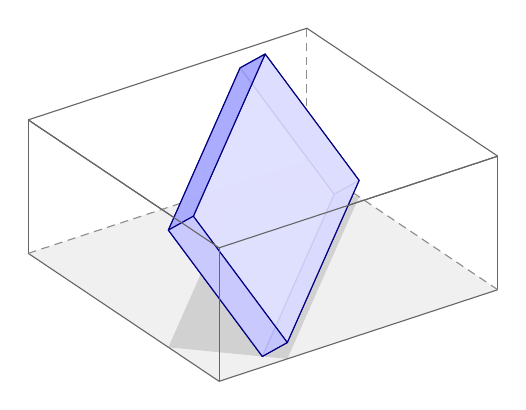
\begin{tikzpicture}[line join=round]
\fill[black!6] (0.000,0.000) -- (3.539,1.163) -- (1.115,2.788) -- (-2.424,1.625) -- cycle;
\fill[black!18] (-0.644,0.432) -- (-0.327,0.401) -- (0.866,0.285) -- (1.778,2.344) -- (0.267,2.491) -- cycle;
\draw[black!60] (0.000,0.000) -- (0.000,1.695);
\draw[black!60] (0.000,0.000) -- (-2.424,1.625);
\draw[black!60] (0.000,0.000) -- (3.539,1.163);
\draw[black!60] (0.000,1.695) -- (-2.424,3.320);
\draw[black!60] (0.000,1.695) -- (3.539,2.859);
\draw[black!60] (-2.424,1.625) -- (-2.424,3.320);
\draw[densely dashed, black!45] (-2.424,1.625) -- (1.115,2.788);
\draw[black!60] (-2.424,3.320) -- (1.115,4.484);
\draw[black!60] (3.539,1.163) -- (3.539,2.859);
\draw[densely dashed, black!45] (3.539,1.163) -- (1.115,2.788);
\draw[black!60] (3.539,2.859) -- (1.115,4.484);
\draw[densely dashed, black!45] (1.115,2.788) -- (1.115,4.484);
\filldraw[fill=blue!22, draw=blue!50!black, fill opacity=0.9] (1.778,2.551) -- (0.585,4.156) -- (0.267,3.980) -- (1.461,2.375) -- cycle;
\filldraw[fill=blue!35, draw=blue!50!black, fill opacity=0.9] (0.866,0.492) -- (1.778,2.551) -- (1.461,2.375) -- (0.549,0.316) -- cycle;
\filldraw[fill=blue!12, draw=blue!50!black, fill opacity=0.9] (0.549,0.316) -- (1.461,2.375) -- (0.267,3.980) -- (-0.644,1.920) -- cycle;
\filldraw[fill=blue!12, draw=blue!50!black, fill opacity=0.9] (0.866,0.492) -- (1.778,2.551) -- (0.585,4.156) -- (-0.327,2.096) -- cycle;
\filldraw[fill=blue!35, draw=blue!50!black, fill opacity=0.9] (-0.327,2.096) -- (0.585,4.156) -- (0.267,3.980) -- (-0.644,1.920) -- cycle;
\filldraw[fill=blue!22, draw=blue!50!black, fill opacity=0.9] (0.866,0.492) -- (-0.327,2.096) -- (-0.644,1.920) -- (0.549,0.316) -- cycle;
\draw[black!60] (0.000,0.000) -- (0.000,1.695);
\draw[black!60] (0.000,1.695) -- (-2.424,3.320);
\draw[black!60] (0.000,1.695) -- (3.539,2.859);
\end{tikzpicture}
\caption{A box $2.8\times1.3\times0.25$ in a container of height $1.2$ with floor $2.7\times2.64$, placed as described by one of the checks of the criterion: the long edge is horizontal, the face $1.3\times0.25$ is tilted in the vertical strip, and the orthogonal projection of the box onto the floor (the shadow) is a $2.8\times h^*$ rectangle rotated in the floor. The rotation is computed as in the proof of Proposition~\ref{prop:suff}.}\label{fig:box}
\end{figure}

\begin{theorem}[Main theorem]\label{thm:main}
Let $p_1,p_2,p_3>0$ and $q_1,q_2,q_3\ge 0$. The box $Q$ fits into the box $P$ if and only if
$\NC(p,q)$ holds.
\end{theorem}

Sufficiency is constructive (Section~\ref{sec:suff}): every check that holds yields an explicit
rotation. Necessity rests on the following theorem (Section~\ref{sec:descent}), which is the main new
ingredient. Here $w_i(R)=\sum_j q_j\abs{R_{ij}}$ is the width of the rotated box along axis $i$
(Section~\ref{sec:widths}).

\begin{theorem}[Descent]\label{thm:Z}
Let $q_1,q_2,q_3>0$ and let $R\in\Ort$ have no zero entries. Then there is $R'\in\Ort$ with
$w_i(R')<w_i(R)$ for $i=1,2,3$.
\end{theorem}

\subsection*{Formal verification}
Theorem~\ref{thm:main} has been formalized and checked in Lean~4 with Mathlib; see
Section~\ref{sec:lean}. The formal statement uses literally the formulas above; the only definitions
on which its meaning depends are those of a box and of fitting.

\section{Reduction to widths}\label{sec:widths}

Every isometry of $\R^3$ has the form $x\mapsto Rx+t$ with $R\in\Ort$ (Mazur--Ulam). Column $j$ of $R$
is the direction of edge $j$ of the moved box, and $R_{ij}$ is the cosine of the angle between this
edge and axis $i$ of $P$.

\begin{lemma}\label{lem:widths}
Let $R$ be any real $3\times3$ matrix. Some translate of $RQ$ lies in $P$ if and only if
\[
w_i(R):=\sum_{j=1}^3 q_j\abs{R_{ij}}\le p_i\qquad(i=1,2,3).
\]
Consequently $Q$ fits into $P$ if and only if $w(R)\le p$ for some $R\in\Ort$.
\end{lemma}

\begin{proof}
The $i$-th coordinate of $Rx=\sum_j R_{ij}x_j$, $x\in Q$, ranges over an interval of length
$\sum_j q_j\abs{R_{ij}}$, the endpoints being attained at vertices of $Q$. The translations along
different axes are independent.
\end{proof}

The same argument in the plane shows that a $u\times v$ rectangle fits into an $a\times b$ rectangle
if and only if $uc+vd\le a$ and $ud+vc\le b$ for some $c,d\ge0$ with $c^2+d^2=1$.

\section{A rectangle in a strip}\label{sec:strip}

Let $x\ge y\ge 0$ and $s\ge0$. For $c,d\ge0$ with $c^2+d^2=1$ put $A=xc+yd$ (the extent of the
rotated $x\times y$ rectangle across the strip) and $B=xd+yc$ (its extent along the strip).

\begin{lemma}[Strip lemma]\label{lem:strip}
\begin{enumerate}
\item[(a)] If $y\le s$, there are $c,d\ge 0$ with $c^2+d^2=1$, $A\le s$ and $B\le H(x,y;s)$.
\item[(b)] If $c,d\ge0$, $c^2+d^2=1$ and $A\le s$, then $y\le s$ and $H(x,y;s)\le B$.
\end{enumerate}
The same holds for arbitrary $u,v\ge0$ in place of $x,y$ with $H(u,v;s)$, $A=uc+vd$, $B=ud+vc$
(exchange $c$ and $d$ if $u<v$).
\end{lemma}

\begin{proof}
If $x=0$ everything is trivial, so let $r=\sqrt{x^2+y^2}>0$ and let $\alpha\in[0,\pi/4]$ be given by
$\cos\alpha=x/r$, $\sin\alpha=y/r$. Write $(c,d)=(\cos\theta,\sin\theta)$ with
$\theta\in[0,\pi/2]$. Then
\[
A(\theta)=r\cos(\theta-\alpha),\qquad B(\theta)=r\sin(\theta+\alpha).
\]
For $\theta\in[0,\pi/2]$ we have $\theta-\alpha\in[-\pi/2,\pi/2]$ and $\theta+\alpha\in[0,\pi]$, so
both $A$ and $B$ are concave on $[0,\pi/2]$; hence on every subinterval they attain their minima at
the endpoints. Moreover $A(0)=B(\pi/2)=x$ and $A(\pi/2)=B(0)=y$.

By concavity $A\ge\min(x,y)=y$, which proves the first claim of (b). If $x\le s$, the angle $\theta=0$
is admissible with $B(0)=y$, and $B\ge\min(B(0),B(\pi/2))=y$ everywhere; this proves both (a) and (b).

Let $y\le s<x$. On $[0,\alpha]$ the function $A$ increases from $x$ to $r$, so $A>s$ there; on
$[\alpha,\pi/2]$ it decreases from $r$ to $y\le s$. Hence the admissible angles form an interval
$[\theta^*,\pi/2]$ with $A(\theta^*)=s$, and the minimum of the concave function $B$ over it equals
$\min(B(\theta^*),B(\pi/2))=\min(B(\theta^*),x)$. It remains to compute $B(\theta^*)$. With
$\varphi=\theta^*-\alpha\in[0,\pi/2]$ we have $\cos\varphi=s/r$, $\sin\varphi=\sqrt{r^2-s^2}/r$, and
\[
\cos\theta^*=\frac{xs-y\sqrt{r^2-s^2}}{r^2},\qquad
\sin\theta^*=\frac{ys+x\sqrt{r^2-s^2}}{r^2},\qquad
B(\theta^*)=\frac{2xys+(x^2-y^2)\sqrt{r^2-s^2}}{r^2}.
\]
Thus $\min\{B:A\le s\}=H(x,y;s)$, which gives (a) (take the minimizing endpoint) and (b).
\end{proof}

\begin{remark}\label{rem:carver}
By the planar version of Lemma~\ref{lem:widths} and Lemma~\ref{lem:strip}, $\Fit(a,b;u,v)$ holds if
and only if the $u\times v$ rectangle fits into the $a\times b$ rectangle. Carver \cite{Carver1957}
gave another closed form of the same condition: for $u\ge v$, $a\ge b$, $u>a$, $v\le b$ it reads
$\bigl(\tfrac{a+b}{u+v}\bigr)^2+\bigl(\tfrac{a-b}{u-v}\bigr)^2\ge 2$. We do not use Carver's form.
(Numerically the two forms agree on $2\cdot10^5$ random rectangles; see \texttt{tools/box\_fit.py}.)
\end{remark}

\section{Sufficiency}\label{sec:suff}

\begin{proposition}\label{prop:suff}
If a check of $\NC(p,q)$ holds, then $Q$ fits into $P$, and an explicit rotation can be written down.
\end{proposition}

\begin{proof}
Relabeling axes and edges (which permutes rows and columns of $R$) we may assume that the check is
$\NC_{(1,2,3),(1,2,3)}$: $\min(q_2,q_3)\le p_1$ and $\Fit(p_2,p_3;q_1,h^*)$ with $h^*=H(q_2,q_3;p_1)$.
By Lemma~\ref{lem:strip}(a) there are $c_1,d_1\ge0$, $c_1^2+d_1^2=1$, with
\[
q_2c_1+q_3d_1\le p_1,\qquad q_2d_1+q_3c_1\le h^*,
\]
in particular $h^*\ge0$. Applying Lemma~\ref{lem:strip}(a) to the rectangle $q_1\times h^*$ in the
strip of width $p_2$ gives $c_2,d_2\ge 0$, $c_2^2+d_2^2=1$, with
\[
q_1c_2+h^*d_2\le p_2,\qquad q_1d_2+h^*c_2\le H(q_1,h^*;p_2)\le p_3 .
\]
Let
\[
R=\begin{pmatrix}0&c_1&-d_1\\ c_2&-d_1d_2&-c_1d_2\\ d_2&d_1c_2&c_1c_2\end{pmatrix}.
\]
Its columns $f_1=(0,c_2,d_2)$, $f_2=c_1e_1+d_1n$, $f_3=-d_1e_1+c_1n$ with $n=(0,-d_2,c_2)$ are
orthonormal, so $R\in\Ort$. Its widths are
\begin{align*}
w_1&=q_2c_1+q_3d_1\le p_1,\\
w_2&=q_1c_2+d_2(q_2d_1+q_3c_1)\le q_1c_2+d_2h^*\le p_2,\\
w_3&=q_1d_2+c_2(q_2d_1+q_3c_1)\le q_1d_2+c_2h^*\le p_3,
\end{align*}
and Lemma~\ref{lem:widths} concludes the proof.
\end{proof}

\section{Positions with a horizontal edge}\label{sec:zero}

\begin{proposition}\label{prop:zero}
Let $q\ge0$, $p>0$, and let $R\in\Ort$ satisfy $w(R)\le p$ and $R_{ij}=0$ for some $i,j$. Then
$\NC(p,q)$ holds.
\end{proposition}

\begin{proof}
Relabeling, let $R_{11}=0$. For an orthogonal matrix $R=(\det R)\operatorname{cof}(R)$ and
$\det R=\pm1$, so each $\abs{R_{ab}}$ equals the absolute value of the corresponding cofactor. Since
$R_{11}=0$, this gives
\[
\abs{R_{22}}=\abs{R_{13}}\abs{R_{31}},\quad \abs{R_{23}}=\abs{R_{12}}\abs{R_{31}},\quad
\abs{R_{32}}=\abs{R_{13}}\abs{R_{21}},\quad \abs{R_{33}}=\abs{R_{12}}\abs{R_{21}}.
\]
Put $c=\abs{R_{12}}$, $d=\abs{R_{13}}$, $c'=\abs{R_{21}}$, $d'=\abs{R_{31}}$; then
$c^2+d^2=1$ (first row) and $c'^2+d'^2=1$ (first column). With $B:=q_2d+q_3c$ we obtain
\[
w_1=q_2c+q_3d,\qquad w_2=q_1c'+d'B,\qquad w_3=q_1d'+c'B .
\]
From $w_1\le p_1$ and Lemma~\ref{lem:strip}(b), $\min(q_2,q_3)\le p_1$ and $h^*:=H(q_2,q_3;p_1)\le B$;
also $h^*\ge0$ by Lemma~\ref{lem:strip}(a). Hence $q_1c'+d'h^*\le w_2\le p_2$ and
$q_1d'+c'h^*\le w_3\le p_3$. Lemma~\ref{lem:strip}(b), applied to the rectangle $q_1\times h^*$ in
the strip of width $p_2$ with direction $(c',d')$, gives $\min(q_1,h^*)\le p_2$ and
$H(q_1,h^*;p_2)\le q_1d'+h^*c'\le p_3$, i.e.\ $\Fit(p_2,p_3;q_1,h^*)$. Thus
$\NC_{(1,2,3),(1,2,3)}$ holds.
\end{proof}

\section{Descent: proof of Theorem~\ref{thm:Z}}\label{sec:descent}

Throughout this section $q_1,q_2,q_3>0$ and $R\in\Ort$ has no zero entries. We write $e_1,e_2,e_3$
for the standard basis, $u\cdot v$ for the scalar product and $u\times v$ for the vector product.

\subsection{Linearization}
Let $s_{ij}=\sgn R_{ij}\in\{\pm1\}$, $g_i=(s_{i1}q_1,s_{i2}q_2,s_{i3}q_3)$ and $a_i=Rg_i\in\R^3$.
Write $A_{ik}=(a_i)_k$. Then $A_{ii}=\sum_j R_{ij}s_{ij}q_j=w_i(R)$. If $C\in\Ort$ and $CR$ has the
same sign pattern as $R$, then
\begin{equation}\label{eq:lin}
w_i(CR)=\sum_j q_j s_{ij}(CR)_{ij}=(Ca_i)_i .
\end{equation}

\begin{lemma}[B1]\label{lem:B1}
$\abs{A_{ik}}<A_{kk}$ for $i\neq k$.
\end{lemma}
\begin{proof}
$\abs{A_{ik}}=\abs{\sum_j s_{ij}q_jR_{kj}}\le\sum_jq_j\abs{R_{kj}}=A_{kk}$. Equality would force all
$s_{ij}R_{kj}$ ($q_j>0$, $R_{kj}\ne0$) to have the same sign, hence all products $R_{ij}R_{kj}$ to be
nonzero of the same sign, contradicting the orthogonality of rows $i$ and $k$.
\end{proof}

\subsection{The Cayley rotation}
For $v\in\R^3$ let $[v]_\times x=v\times x$ and
\[
C(v)=\frac{(1-\abs{v}^2)I+2[v]_\times+2vv^{\mathsf T}}{1+\abs{v}^2}.
\]
This is the rotation given by the quaternion $(1,v)$; one checks directly that $C(v)C(v)^{\mathsf T}=I$.
Moreover $C(0)=I$ and $C$ is continuous. For $a\in\R^3$ put
\[
b_i(a)=a\times e_i,\qquad P_i(a;v)=v_i\,(v\cdot a)-\abs{v}^2a_i,\qquad D_i(a;v)=b_i(a)\cdot v+P_i(a;v).
\]
Since $e_i\cdot(v\times a)=v\cdot(a\times e_i)$, a direct computation gives
\begin{equation}\label{eq:cay}
(C(v)a)_i-a_i=\frac{2}{1+\abs{v}^2}\,D_i(a;v).
\end{equation}
Note that $P_i(a;\cdot)$ is a quadratic form: $P_i(a;tv)=t^2P_i(a;v)$. This is why we use the Cayley
parametrization: by \eqref{eq:cay} the change of each width is, up to a positive factor, an explicit
polynomial of degree two in $v$, so both its first- and second-order terms are available.

\subsection{Descent along a curve}
We shall rotate along $v(t)=t(h+tz)$, $t>0$ small. Then
\begin{equation}\label{eq:curve}
D_i(a;v(t))=t\,b_i(a)\cdot h+t^2\bigl(b_i(a)\cdot z+P_i(a;h+tz)\bigr).
\end{equation}

\begin{lemma}\label{lem:order}
Let $a,h,z\in\R^3$ and $b=b_i(a)$.
\begin{enumerate}
\item[(a)] If $b\cdot h<0$, or $b\cdot h=0$ and $b\cdot z+P_i(a;h)<0$, then $D_i(a;v(t))<0$ for all
sufficiently small $t>0$.
\item[(b)] If $b=0$, $a_i>0$ and all components of $z$ are nonzero, then $D_i(a;v(t))<0$ for all
sufficiently small $t>0$.
\end{enumerate}
\end{lemma}
\begin{proof}
(a) By \eqref{eq:curve}, $D_i/t=b\cdot h+t(b\cdot z+P_i(a;h+tz))\to b\cdot h$ as $t\to0^+$; in the
second case $D_i/t^2=b\cdot z+P_i(a;h+tz)\to b\cdot z+P_i(a;h)$.
(b) $b=a\times e_i=0$ means $a=a_ie_i$; then $P_i(a;u)=u_i^2a_i-\abs{u}^2a_i=-a_i\sum_{m\ne i}u_m^2$.
For small $t>0$ every component $h_m+tz_m$ of $u=h+tz$ is nonzero (if $h_m\ne0$ by continuity, if
$h_m=0$ because $z_m\ne0$). Hence $D_i(a;v(t))=t^2P_i(a;h+tz)<0$.
\end{proof}

\subsection{The key inequality}

\begin{lemma}\label{lem:key}
Let $a_1,a_2,a_3\in\R^3$ satisfy $\abs{A_{ik}}<A_{kk}$ for $i\ne k$, where $A_{ik}=(a_i)_k$. Let
$\nu\in\R^3$, $\nu\ge0$, have at least two positive entries and satisfy
$\sum_i\nu_i\,b_i(a_i)=0$. Then $\sum_i\nu_iP_i(a_i;h)<0$ for every $h\ne0$.
\end{lemma}

\begin{proof}
Since $a\times e_1=(0,a_3,-a_2)$, $a\times e_2=(-a_3,0,a_1)$, $a\times e_3=(a_2,-a_1,0)$, the condition
$\sum_i\nu_ib_i(a_i)=0$ says precisely that
\[
\nu_iA_{ik}=\nu_kA_{ki}\qquad(i\ne k).
\]
Put $d_i=\nu_iA_{ii}\ge0$ and $m_{ik}=\nu_iA_{ik}=\nu_kA_{ki}$. Expanding and using the symmetry,
\[
\sum_i\nu_iP_i(a_i;h)=\sum_i\nu_i\Bigl(h_i\sum_kh_kA_{ik}-\abs{h}^2A_{ii}\Bigr)=-\sum_{i<k}B_{ik},
\qquad B_{ik}=d_ih_k^2+d_kh_i^2-2m_{ik}h_ih_k .
\]
By the hypothesis,
$m_{ik}^2=\nu_i\nu_kA_{ik}A_{ki}\le\nu_i\nu_k\abs{A_{ik}}\abs{A_{ki}}\le\nu_i\nu_kA_{kk}A_{ii}=d_id_k$,
with strict inequality if $\nu_i\nu_k>0$.

Each $B_{ik}\ge0$: if $d_i=0$ then $m_{ik}=0$ and $B_{ik}=d_kh_i^2$; if $d_i>0$ then
$d_iB_{ik}=(d_ih_k-m_{ik}h_i)^2+(d_id_k-m_{ik}^2)h_i^2\ge0$.

Some $B_{ik}$ is positive. Choose $c$ with $h_c\ne0$ and, using the two positive entries of $\nu$, an
index $i\ne c$ with $\nu_i>0$, so $d_i>0$. If $d_c=0$ then $m_{ic}=0$ and $B_{ic}=d_ih_c^2>0$. If
$d_c>0$ then $\nu_c>0$, hence $m_{ic}^2<d_id_c$, and $d_iB_{ic}=(d_ih_c-m_{ic}h_i)^2+(d_id_c-m_{ic}^2)h_i^2$
is positive both for $h_i\ne0$ and for $h_i=0$.
\end{proof}

\subsection{Choice of the curve}
The idea is as follows. Either some direction $h$ decreases all widths to first order, or the
first-order terms $b_i\cdot h$ are blocked by a nonnegative relation $\sum_i\nu_ib_i=0$; in the latter
case Lemma~\ref{lem:key} shows that the second-order terms decrease the widths.
We use Motzkin's theorem of the alternative \cite{Motzkin1936,Schrijver1986} in the following form:
for vectors $b_i\in\R^3$ and numbers $c_i$, $i\in K$, either the system $b_i\cdot z<c_i$ ($i\in K$)
has a solution, or there is $\mu\ge0$, $\mu\ne0$, supported on $K$, with $\sum_i\mu_ib_i=0$ and
$\sum_i\mu_ic_i\le0$.

\begin{lemma}\label{lem:choice}
Let $a_i$ be as in the Linearization, $b_i=b_i(a_i)$ and $K=\{i:b_i\ne0\}$. There are $h,z\in\R^3$
such that all components of $z$ are nonzero and, for each $i\in K$, either $b_i\cdot h<0$, or
$b_i\cdot h=0$ and $b_i\cdot z+P_i(a_i;h)<0$.
\end{lemma}

\begin{proof}
Apply Motzkin's theorem with $c=0$. If $b_i\cdot h<0$ for all $i\in K$ has a solution $h$, take
$z=(1,1,1)$. Otherwise there is $\mu\ne0$, $\mu\ge0$, with $\sum\mu_ib_i=0$ (note $b_i=0$ for
$i\notin K$), so the matrix with rows $b_1,b_2,b_3$ is singular and there is $h\ne0$ with $b_i\cdot h=0$
for all $i$. Apply Motzkin's theorem again, with $c_i=-P_i(a_i;h)$.

If there is $z_0$ with $b_i\cdot z_0+P_i(a_i;h)<0$ for $i\in K$, then $z=z_0+\delta(1,1,1)$ with small
$\delta>0$ keeps these strict inequalities and has all components nonzero.

Otherwise there is $\nu\ge0$, $\nu\ne0$, supported on $K$, with $\sum\nu_ib_i=0$ and
$\sum\nu_iP_i(a_i;h)\ge0$. If $\nu$ had a single positive entry $\nu_i$, then $\nu_ib_i=0$ would give
$b_i=0$, contradicting $i\in K$. So $\nu$ has two positive entries, and Lemma~\ref{lem:key} (whose
hypothesis holds by Lemma~\ref{lem:B1}) gives $\sum\nu_iP_i(a_i;h)<0$, a contradiction.
\end{proof}

\subsection{Proof of Theorem~\ref{thm:Z}}
Take $h,z$ from Lemma~\ref{lem:choice} and put $R(t)=C(v(t))R$. For all sufficiently small $t>0$:
\begin{itemize}
\item $R(t)\in\Ort$ has the same sign pattern as $R$, because $R(t)\to R$ and $R$ has no zero entries;
\item $D_i(a_i;v(t))<0$ for each $i$: for $i\in K$ by Lemma~\ref{lem:order}(a), and for $i\notin K$ by
Lemma~\ref{lem:order}(b), since $(a_i)_i=w_i(R)>0$.
\end{itemize}
By \eqref{eq:lin} and \eqref{eq:cay},
$w_i(R(t))-w_i(R)=(C(v(t))a_i)_i-(a_i)_i=\frac{2}{1+\abs{v(t)}^2}D_i(a_i;v(t))<0$ for $i=1,2,3$.
\qed

\section{Proof of the main theorem}\label{sec:proof}

Sufficiency is Proposition~\ref{prop:suff}. For necessity, by Proposition~\ref{prop:zero} it suffices
to show: \emph{if $Q$ fits into $P$, then $w(R)\le p$ for some $R\in\Ort$ with a zero entry.}

\emph{Case $q_1,q_2,q_3>0$.} The function $F(R)=\max_iw_i(R)/p_i$ is continuous on the compact group
$\Ort$ and attains its minimum at some $R^*$; since $Q$ fits, $F(R^*)\le1$, i.e.\ $w(R^*)\le p$. If
$R^*$ had no zero entries, Theorem~\ref{thm:Z} would give $R'$ with $w_i(R')<w_i(R^*)$ for all $i$,
hence $F(R')<F(R^*)$. So $R^*$ has a zero entry.

\emph{General case $q\ge0$.} Let $w(R_0)\le p$ and suppose that no $R$ in the compact set
$Z=\{R\in\Ort:\ R_{ij}=0\text{ for some }i,j\}$ satisfies $w(R)\le p$. Then the continuous function
$\varphi(R)=\max_i(w_i(R)-p_i)$ is positive on $Z$ and has a minimum $m>0$ there. Let $\delta=m/6$,
$q'=q+\delta(1,1,1)>0$ and $p'=p+3\delta(1,1,1)$. Since $\sum_j\abs{R_{ij}}\le3$ for $R\in\Ort$, we
have $w_i(R_0;q')=w_i(R_0;q)+\delta\sum_j\abs{(R_0)_{ij}}\le p_i'$, so $q'$ fits into $p'$. By the
previous case there is $R_1\in Z$ with $w(R_1;q')\le p'$, hence $w_i(R_1;q)\le w_i(R_1;q')\le p_i+3\delta$
and $\varphi(R_1)\le3\delta<m$, a contradiction. \qed

\section{Examples}\label{sec:examples}

\begin{example}[A rod]
Let $q=(L,0,0)$. Take the check with height $i=1$, horizontal edge $j=2$ and $(k,l)=(1,3)$. Then
$h^*=H(L,0;p_1)=\sqrt{\max(L^2-p_1^2,0)}$, and $\Fit(p_2,p_3;0,h^*)$ reduces to $h^{*2}\le p_2^2+p_3^2$.
Thus the check holds if and only if $L^2\le p_1^2+p_2^2+p_3^2$; conversely, a longer rod cannot fit
since $\sqrt{p_1^2+p_2^2+p_3^2}$ is the diameter of $P$. The rod fits exactly along the space
diagonal, and this position has an edge (of length $0$) perpendicular to an axis.
\end{example}

\begin{example}[A square in a cube]
The largest square that fits into the unit cube has side $a=3\sqrt2/4$ (Nieuwland, published by van Swinden
\cite{vanSwinden1816}). For $q=(a,a,0)$ and $p=(1,1,1)$ take $j=1$, $(k,l)=(2,3)$: $h^*=H(a,0;1)=
\sqrt{a^2-1}=\sqrt2/4$. For the floor, $x^2=9/8$, $y^2=1/8$, $x^2+y^2=5/4$, $\sqrt{x^2+y^2-1}=1/2$,
$2xy=3/4$, so the second branch of \eqref{eq:H} equals $(3/4+1\cdot\tfrac12)/(5/4)=1$ and
$H(a,h^*;1)=\min(a,1)=1$: the check holds with equality, in accordance with Nieuwland's result.
\end{example}

\begin{example}[Classical necessary conditions are not sufficient]
For $p=(1,1,1)$ and $q=(1.1,1.1,0.01)$ the sums of edges, of squared edges, the surface areas and the
volumes are all smaller for $Q$, yet $Q$ does not fit: its $1.1\times1.1$ face would give a square
larger than $3\sqrt2/4$ in the cube.
\end{example}

\section{Computation}\label{sec:computation}

The criterion consists of at most $36$ evaluations of formula~\eqref{eq:H} and comparisons, so it takes
constant time. When a check holds, the proof of Proposition~\ref{prop:suff} gives the rotation
explicitly: two angles from Lemma~\ref{lem:strip}(a), one for the face in the vertical strip and one
for the rectangle on the floor. The reference implementation \texttt{tools/box\_fit.py} in the
repository (Section~\ref{sec:lean}) returns a rotation matrix $R$ with $\det R=1$ and a translation
$t$ such that $x\mapsto Rx+t$ maps $Q$ into $P$; its self-test verifies about $2\cdot10^4$ random
placements (orthogonality of $R$ and all vertices inside $P$).

For comparison we used a numerical search that minimises $\max_iw_i(R)/p_i$ over rotations by the
Nelder--Mead method from random starts and answers ``fits'' when some start reaches a value $\le1$.
On $200$ random pairs near the boundary (the box scaled by a factor $1\pm e$ from the largest fitting
size, $10^{-4}\le e\le10^{-2}$) the criterion takes about $24$ microseconds per pair and the explicit
placement about $20$ microseconds (Python, one core of a desktop computer), while the numerical
search takes $78$, $228$ and $517$ milliseconds per pair with $5$, $20$ and $50$ starts, i.e.\ it is
$3\cdot10^3$ to $2\cdot10^4$ times slower, and gives $27$, $5$ and $0$ wrong answers respectively. All
its errors are ``does not fit'' for boxes that fit: a local search can confirm that a box fits, but its
failure to find a position proves nothing. A rigorous negative answer requires a global method with
guaranteed bounds, such as a branch-and-bound search over rotations, which is considerably more
expensive; the criterion gives both answers exactly. The script is \texttt{tools/benchmark.py}.

\section{Strict fitting}\label{sec:strict}

\begin{remark}\label{rem:strict}
Say that $Q$ \emph{fits strictly} into $P$ if $f(Q)$ lies in the open box
$(0,p_1)\times(0,p_2)\times(0,p_3)$ for some isometry $f$, i.e.\ without touching the boundary of $P$.
Let $H^\circ$ be defined as $H$ in \eqref{eq:H}, but with the case split $x<s$ / $x\ge s$ instead of
$x\le s$ / $x>s$, and let $\NC^\circ$ be the criterion of Definition~\ref{def:NC} in which all
inequalities are strict and $H$ is replaced by $H^\circ$. Then, for $p>0$ and $q\ge0$:
\begin{itemize}
\item $Q$ fits strictly into $P$ if and only if $\NC(p-\varepsilon(1,1,1),q)$ holds for some
$0<\varepsilon<\min_ip_i$;
\item $Q$ fits strictly into $P$ if and only if $\NC^\circ(p,q)$ holds.
\end{itemize}
Complete formal proofs are in \texttt{lean/Boxes/Strict.lean} (theorems
\texttt{fitsStrict\_iff\_shrink} and \texttt{fitsStrict\_iff\_NCs}); they follow
Sections~\ref{sec:widths}--\ref{sec:proof} with strict inequalities.

The change of the case split is essential, because $H(x,y;s)$ jumps at $s=x$: a face whose longer side
equals the height may stand upright touching the ceiling, but if touching is forbidden it cannot be
tilted slightly (a small tilt increases its height). For example, let $p=(1,1,1)$ and
$q=(1,0.5,0.5)$. Making only the inequalities strict gives a check that holds: with a horizontal edge
$0.5$, $h^*=H(1,0.5;1)=0.5$ and $0.5\times0.5$ fits strictly into $1\times1$. But $\NC^\circ$ fails:
here $H^\circ(1,0.5;1)=\min\bigl(1,\,0.5\cdot2.75/1.25\bigr)=1$, and each check requires
$H^\circ(1,0.5;1)<1$ (for the floor if the horizontal edge is $1$, and for $h$ and then the floor if it
is $0.5$). So this box does not fit strictly.
\end{remark}

\section{Formal verification}\label{sec:lean}

The accompanying repository \url{https://github.com/MikhailLevit1987/box-in-box} (archived at Zenodo, \href{https://doi.org/10.5281/zenodo.22974798}{doi:10.5281/zenodo.22974798}) contains a Lean~4 formalization (Lean v4.34.0-rc2, Mathlib) of
Theorem~\ref{thm:main} and of the statements of Remark~\ref{rem:strict}, about 1800 lines in seven
files:
\begin{itemize}
\item \texttt{Reduction.lean}, \texttt{Statement.lean}: definitions, Lemma~\ref{lem:widths} (via
Mazur--Ulam), Lemma~\ref{lem:strip}(a), Proposition~\ref{prop:suff};
\item \texttt{ZeroEntry.lean}: Lemma~\ref{lem:strip}(b) (by a chord argument instead of concavity),
Proposition~\ref{prop:zero};
\item \texttt{Motzkin.lean}: the theorem of the alternative (via Hahn--Banach separation);
\item \texttt{Descent.lean}: Section~\ref{sec:descent};
\item \texttt{Necessity.lean}: Section~\ref{sec:proof} and the main theorem \texttt{fits\_iff\_NC};
\item \texttt{Strict.lean}: Section~\ref{sec:strict}, theorems \texttt{fitsStrict\_iff\_shrink} and
\texttt{fitsStrict\_iff\_NCs} (with two further definitions, the open box and strict fitting).
\end{itemize}
The statement and the two definitions on which its meaning depends read verbatim:
\begin{verbatim}
def box (q : Fin 3 → ℝ) : Set E3 := {x | ∀ i, 0 ≤ x i ∧ x i ≤ q i}
def Fits (p q : Fin 3 → ℝ) : Prop := ∃ f : E3 ≃ᵢ E3, f '' box q ⊆ box p
theorem fits_iff_NC (p q : Fin 3 → ℝ) (hp : ∀ i, 0 < p i) (hq : ∀ i, 0 ≤ q i) :
    Fits p q ↔ NC p q
\end{verbatim}
Here \texttt{E3} is the Euclidean space $\R^3$, \texttt{box q} is the set of points $x$ with
$0\le x_i\le q_i$, and \texttt{Fits p q} means that some isometry $f$ of $\R^3$ maps \texttt{box q}
into \texttt{box p}. The criterion \texttt{NC} is Definition~\ref{def:NC} verbatim (with indices
$0,1,2$). The command \texttt{\#print axioms Boxes.fits\_iff\_NC} reports only the standard axioms
\texttt{propext}, \texttt{Classical.choice}, \texttt{Quot.sound}.

\begin{thebibliography}{99}
\bibitem{AlexanderWetzel2005} R.~Alexander, J.~E.~Wetzel, Wafer in a box, \emph{Math. Mag.} 78 (2005) 214--220.
\bibitem{Carver1925} W.~B.~Carver, Solution of Problem 3036, \emph{Amer. Math. Monthly} 32 (1925) 47--49.
\bibitem{Carver1957} W.~B.~Carver, Solution of Problem E1225, \emph{Amer. Math. Monthly} 64 (1957) 114--116.
\bibitem{Garnett1923} F.~M.~Garnett, Problem 3036, \emph{Amer. Math. Monthly} 30 (1923) 337.
\bibitem{JerrardWetzel2004} R.~P.~Jerrard, J.~E.~Wetzel, Prince Rupert's rectangles, \emph{Amer. Math. Monthly} 111 (2004) 22--31.
\bibitem{JSSW2006} R.~Jerrard, J.~Schneider, R.~Smallberg, J.~Wetzel, Straw in a box, \emph{College Math. J.} 37 (2006) 93--102.
\bibitem{Kvant1999} Problem M1687 (Tournament of Towns, 1998), \emph{Kvant} 1999, no.~6, p.~16 (in Russian).
\bibitem{MartinStephenson1989} R.~R.~Martin, P.~C.~Stephenson, Containment algorithms for objects in rectangular boxes, in: \emph{Theory and Practice of Geometric Modeling}, Springer, 1989, 307--325.
\bibitem{Motzkin1936} T.~S.~Motzkin, \emph{Beitr\"age zur Theorie der linearen Ungleichungen}, Dissertation, Basel, 1936.
\bibitem{Post1993} K.~A.~Post, Triangle in a triangle: on a problem of Steinhaus, \emph{Geom. Dedicata} 45 (1993) 201--225.
\bibitem{Schrijver1986} A.~Schrijver, \emph{Theory of Linear and Integer Programming}, Wiley, 1986.
\bibitem{vanSwinden1816} J.~H.~van Swinden, \emph{Grondbeginsels der Meetkunde}, 2nd ed., Amsterdam, 1816.
\bibitem{Wetzel2000} J.~E.~Wetzel, Rectangles in rectangles, \emph{Math. Mag.} 73 (2000) 204--211.
\end{thebibliography}

\end{document}
